
\documentclass[conference]{IEEEtran}
\usepackage{times}
\usepackage{color}

% numbers option provides compact numerical references in the text.
\usepackage[numbers]{natbib}
\usepackage{multicol}
\usepackage[bookmarks=true]{hyperref}
\usepackage{amsmath}
\usepackage{graphicx}
\usepackage[export]{adjustbox}
\usepackage{subcaption}
\usepackage{caption}
\usepackage{wrapfig}
\usepackage{verbatim}
\usepackage{color}
\usepackage{url}

\pdfinfo{
   /Author (Anonymous)
   /Title  (End-to-End Training of Deep Visuomotor Policies)
   /Subject (policy search)
   /Keywords (policy search;reinforcement learning;optimal control;vision;neural networks)
}

%% editing comment
\newcommand{\cmt}[1]{{\footnotesize\textcolor{red}{#1}}}
\newcommand{\note}[1]{\cmt{Note: #1}}
\newcommand{\todo}[1]{\cmt{TO-DO: #1}}
\newcommand{\nopphon}[1]{\cmt{Nopphon: #1}}
\newcommand{\chelsea}[1]{\cmt{Chelsea: #1}}
\newcommand{\justin}[1]{\cmt{Justin: #1}}

%% ignore text
\long\def\ignorethis#1{}

%% abbreviations
\newcommand{\etal}{{et~al.}\ }
\newcommand{\eg}{e.g.\ }
\newcommand{\ie}{i.e.\ }
\newcommand{\nth}{\text{th}}
\newcommand{\pr}{^\prime}
\newcommand{\tr}{^\mathrm{T}}
\newcommand{\inv}{^{-1}}
\newcommand{\pinv}{^{\dagger}}
\newcommand{\real}{\mathbb{R}}
\newcommand{\gauss}{\mathcal{N}}
\newcommand{\norm}[1]{\left|#1\right|}
\newcommand{\trace}{\text{tr}}

%% reference shortcuts
\newcommand{\figtodo}[1]{\framebox[0.8\columnwidth]{\rule{0pt}{1in}#1}}
\newcommand{\figref}[1]{Figure~\ref{fig:#1}}
%\renewcommand{\eqref}[1]{Equation~(\ref{eq:#1})}
\newcommand{\secref}[1]{Section~\ref{sec:#1}}

%% section definitions.
\newcommand{\secpaperlin}{5.1}
\newcommand{\eqnpapergradmul}{3}
\newcommand{\eqnpapergrads}{4}
\newcommand{\applinhess}{A}
\newcommand{\applqr}{B}
\newcommand{\appfastgrad}{C}

%% general math definitions
\newcommand{\vnorm}[1]{\|#1\|}
\newcommand{\lscnorm}[1]{\ell_{12}(#1)}
\newcommand{\costnorm}{r_\ell}
\newcommand{\channel}{c}
\newcommand{\softmax}{\mathbf{s}}
\newcommand{\softmaxpix}{s_{cij}}
\newcommand{\responsemap}{\mathbf{a}}
\newcommand{\responsepix}{a_{cij}}
\newcommand{\responsepixprime}{a_{ci'j'}}



\begin{document}

% paper title
\title{Robust Object Pose Tracking for Robotics}


\author{\authorblockN{Chelsea Finn}
%\authorblockA{School of Electrical and\\Computer Engineering\\
%Atlanta, Georgia 30332--0250\\
%Email: mshell@ece.gatech.edu}
\and
\authorblockN{Justin Fu}
%\authorblockA{Twentieth Century Fox\\
%Email: homer@thesimpsons.com}
\and
\authorblockN{Nopphon Siranart}
%\authorblockA{Starfleet Academy\\
}}

% avoiding spaces at the end of the author lines is not a problem with
% conference papers because we don't use \thanks or \IEEEmembership


% for over three affiliations, or if they all won't fit within the width
% of the page, use this alternative format:
%
%\author{\authorblockN{Michael Shell\authorrefmark{1},
%Homer Simpson\authorrefmark{2},
%James Kirk\authorrefmark{3},
%Montgomery Scott\authorrefmark{3} and
%Eldon Tyrell\authorrefmark{4}}
%\authorblockA{\authorrefmark{1}School of Electrical and Computer Engineering\\
%Georgia Institute of Technology,
%Atlanta, Georgia 30332--0250\\ Email: mshell@ece.gatech.edu}
%\authorblockA{\authorrefmark{2}Twentieth Century Fox, Springfield, USA\\
%Email: homer@thesimpsons.com}
%\authorblockA{\authorrefmark{3}Starfleet Academy, San Francisco, California 96678-2391\\
%Telephone: (800) 555--1212, Fax: (888) 555--1212}
%\authorblockA{\authorrefmark{4}Tyrell Inc., 123 Replicant Street, Los Angeles, California 90210--4321}}


\maketitle

\begin{abstract}

Policy search methods based on reinforcement learning and optimal control can allow robots to automatically learn a wide range of tasks. However, practical applications of policy search tend to require the policy to be supported by hand-engineered components for perception, state estimation, and low-level control. We propose a method for learning policies that map raw, low-level observations, consisting of joint angles and camera images, directly to the torques at the robot's joints. The policies are represented as deep convolutional neural networks (CNNs) with 92,000 parameters. The high dimensionality of such policies poses a tremendous challenge for policy search. To address this challenge, we develop a sensorimotor guided policy search method that can handle high-dimensional policies and partially observed tasks. We use BADMM to decompose policy search into an optimal control phase and supervised learning phase, allowing CNN policies to be trained with standard supervised learning techniques. This method can learn a number of manipulation tasks that require close coordination between vision and control, including inserting a block into a shape sorting cube, screwing on a bottle cap, fitting the claw of a toy hammer under a nail with various grasps, and placing a coat hanger on a clothes rack.

%We address this challenge with a new sensorimotor guided policy search method, which uses BADMM to decompose policy search into a trajectory-centric optimal control phase and supervised learning phase, allowing complex, high-dimensional policies to be trained with standard supervised learning techniques. We show that our method can learn a number of complex manipulation tasks that require close coordination between vision and control, including inserting a block into a shape sorting cube, screwing on a bottle cap, fitting the claw of a toy hammer under a nail with various grasps, and placing a coat hanger on a clothes rack.

\end{abstract}

\IEEEpeerreviewmaketitle

\section{Introduction}
\label{sec:intro}

% In the final version, write a more ambitious introduction that stresses the value of extending deep learning methods to robotic control; consider taking some ideas from Igor's introduction.

Reinforcement learning and policy search methods hold the promise of allowing robots to acquire new behaviors through experience. They have been applied to a range of robotic tasks, including manipulation \cite{drf-lclcm-11,kop-rlarm-10} and locomotion \cite{emmnc-lcbbl-08,gpw-fbwrc-06,kp-pgrlf-04,tzs-spgrl-04}. However, policies learned using such methods often rely on a number of hand-engineered components for perception and low-level control. The policy might specify a trajectory in task-space, relying on hand-designed PD controllers to execute the desired motion, and a policy for manipulating objects might rely on an existing vision system to localize these objects \cite{phas-lgmsl-09}. The vision system in particular can be complex and prone to errors, and its performance is typically not improved during policy training, nor adapted to the goal of the task.

We propose a method for learning policies that directly map raw observations, including joint angles and camera images, to motor torques. The policies are trained end-to-end using real-world experience, optimizing both the control and perception components on the same measure of task performance. This allows the policy to learn goal-driven perception, which avoids the mistakes that are most costly for task performance. Learning perception and control in a general and flexible way requires a large, expressive model. Our policies are represented with convolutional neural networks (CNNs), which have 92,000 parameters and 7 layers. Deep CNN models have been shown to achieve state of the art results on a number of supervised vision tasks \cite{gddm-fhaod-13,ksh-incdc-12,tjlb-jcngm-14}, but sensorimotor deep learning remains a challenging prospect. The policies are extremely high dimensional, and the control task is partially observed, since part of the state must be inferred from images.

\begin{figure}
\setlength{\unitlength}{0.5\columnwidth}
\begin{picture}(1.99,1.15) \linethickness{0.5pt}
%\put(1.3,0.55){\includegraphics[width=0.26\columnwidth]{trial_imgs/hammer_nohold_start.png}}


\put(0.05,0.55){\includegraphics[width=0.28\columnwidth]{trial_imgs/hanger_firstperson_close_step1.png}}
\put(0.05,-0.02){\includegraphics[width=0.28\columnwidth]{trial_imgs/hammer_firstperson_grasp1.png}}
\put(0.62,0.55){\includegraphics[width=0.28\columnwidth]{trial_imgs/traphold1.png}}
\put(0.62,-0.02){\includegraphics[width=0.28\columnwidth]{trial_imgs/bottle_hold_start.png}}

%\put(0.8,0.55){\includegraphics[width=0.28\columnwidth]{imgs/hanger_teaser.png}}
%\put(.8,-0.02){\includegraphics[width=0.28\columnwidth]{imgs/hammer_teaser.png}}
%\put(1.37,0.55){\includegraphics[width=0.28\columnwidth]{imgs/trap_teaser.png}}
%\put(1.37,-0.02){\includegraphics[width=0.28\columnwidth]{imgs/bottle_teaser.png}}

\put(1.19,-0.02){\includegraphics[width=0.368\columnwidth]{imgs/pr2_sm_crop.png}}

\put(0.07,0.0){\textcolor{white}{hammer}}
\put(0.07,0.57){\textcolor{white}{hanger}}
\put(0.64,0.0){\textcolor{white}{bottle}}
\put(0.64,0.57){\textcolor{white}{cube}}

\end{picture}
\caption{Our method learns visuomotor policies that directly use camera image observations (left) to set motor torques on a PR2 robot (right).
%Left: PR2 placing a block into a shape sorting cube.
% using a learned visuomotor policy. Right: images seen by the policy during each task in a visual generalization experiment.
%Right: overlaid sequences of images seen by the policy during generalization tests.
\label{fig:teaser}
}
\vspace{-0.35in}
%\vspace{-0.40in}
\end{figure}

%\begin{figure}
%\setlength{\unitlength}{0.5\columnwidth}
%\begin{picture}(1.99,0.93) \linethickness{0.5pt}
%\put(0.02,-0.00){\includegraphics[width=0.62\columnwidth]{imgs/pr2block_leftside.png}}
%\put(1.08,-0.034){\includegraphics[width=0.448\columnwidth]{imgs/firstperson_block.png}}
%\end{picture}
%\caption{PR2 robot inserting a block into a shape sorting cube using a learned visuomotor policy. The camera image %seen by the policy is shown on the right.
%\label{fig:teaser}
%}
%\vspace{-0.2in}
%\end{figure}

To address these challenges, we extend the framework of guided policy search to sensorimotor deep learning. Guided policy search decomposes the policy learning problem into two phases: a trajectory optimization phase that determines how to solve the task in a few specific conditions, and a supervised learning phase that trains the policy from these successful executions with supervised learning \cite{lk-lcnnp-14}. Since the CNN policy is trained with supervised learning, we can use the tools developed in the deep learning community to make this phase simple and efficient. We handle the partial observability of visuomotor control by optimizing the trajectories with full state information, while providing only partial observations (consisting of images and robot configurations) to the policy. The trajectories are optimized under unknown dynamics, using real-world experience and minimal prior knowledge.

%We use a new, efficient formulation of guided policy search based on the Bregman alternating directions method of multipliers (BADMM) \cite{wb-badmm-14}. Our method handles the partial observability of visuomotor control by optimizing the trajectories with full state information, while providing only partial observations (consisting of images and robot configurations) to the policy. The trajectories are optimized under unknown dynamics, using real-world experience and minimal prior knowledge.

The main contribution of our work is a method for end-to-end training of deep visuomotor policies for robotic manipulation. We propose a partially observed guided policy search algorithm that can train high-dimensional policies for tasks where part of the state must be determined from camera images.
%, efficient formulation of guided policy search that can train high-dimensional policies for partially observed tasks, where part of the state must be determined from camera images.
% based on the Bregman alternating directions method of multipliers (BADMM) \cite{wb-badmm-14}, which can train policies for partially observed tasks where part of the state must be determined from camera images.
We also introduce a novel CNN architecture designed for robotic control, shown in Figure~\ref{fig:nn}. The vision layers of this CNN are designed for localizing points of interest in an image, unlike standard vision architectures that discard locational information to induce translational invariance \cite{ksh-incdc-12}. We evaluate our method by learning policies for inserting a block into a shape sorting cube, screwing a cap onto a bottle, fitting the claw of a toy hammer under a nail with various grasps, and placing a coat hanger on a rack (see Figure~\ref{fig:teaser}). Our results demonstrate clear improvements in consistency and generalization from training visuomotor policies end-to-end, when compared to using the poses or features produced by a CNN trained for 3D object localization.

\section{Related Work}
\label{sec:related}

Reinforcement learning and policy search have been applied in robotics for playing games such as table tennis \cite{kop-rlarm-10}, object manipulation \cite{drf-lclcm-11,phas-lgmsl-09}, and locomotion \cite{emmnc-lcbbl-08,gpw-fbwrc-06,kp-pgrlf-04,tzs-spgrl-04}. Several recent papers provide surveys of policy search in robotics \cite{dnp-spsr-13,kbp-rlrs-13}. Such methods are typically applied to one component of the robot control pipeline, which often sits on top of a hand-designed controller, such as a PD controller, and accepts processed input, for example from an existing vision pipeline \cite{phas-lgmsl-09}. Our method trains policies that map visual input and joint encoder signals directly to the torques at the robot's joints. By learning the entire mapping from perception to control, the perception layers can be adapted to optimize task performance.

We represent our policies with convolutional neural networks (CNNs). CNNs have recently achieved dramatic improvements on a number of vision benchmarks \cite{gddm-fhaod-13,ksh-incdc-12,tjlb-jcngm-14}. Most applications of CNNs focus on classification, where locational information is intentionally discarded by means of successive pooling layers \cite{lgrn-cdbn-09}. Applications to localization typically either use a sliding window to localize the object, reducing the task to classification \cite{gddm-fhaod-13}, perform regression to a heatmap of manually labeled keypoints \cite{tjlb-jcngm-14}, requiring precise knowledge of the object position in the image and camera calibration, or use 3D models to localize previously scanned objects \cite{psgs-3ddpm-12,sl-3dgoc-07}. We use a novel CNN architecture that automatically learns feature points without any supervision beyond the information from the robot's encoders and camera.

Unlike with visual recognition, applications of deep networks to robotic control have been comparatively limited. Backpropagation through the dynamics and the image formation process is impractical, since they are often non-differentiable, and such long-range backpropagation leads to extreme numerical instability. The high dimensionality of the network also makes reinforcement learning very difficult \cite{dnp-spsr-13}. Pioneering early work on neural network control used small, simple networks \cite{hszg-nncss-92,p-alvin-89}, and has largely been supplanted by methods that use carefully designed policies that can be learned efficiently with reinforcement learning \cite{kbp-rlrs-13}. More recent work on sensorimotor deep learning has tackled simple task-space motion \cite{lr-avsrg-13} and used unsupervised learning to obtain low-dimensional state spaces from images \cite{rlv-arlrv-12}, but such methods are limited to tasks with a low-dimensional structure. CNNs have also been trained to play video games with temporal difference learning and Monte Carlo tree search \cite{gsllw-amcts-14,mksga-padrl-13}. However, such methods have only been demonstrated on discrete, synthetic domains, and require an impractical number of samples for real-world robotic applications. Our method is sample efficient, requiring only minutes of interaction time. To the best of our knowledge, this is the first method that can train deep visuomotor policies for complex, high-dimensional manipulation skills with direct torque control.

Learning visuomotor policies end-to-end introduces two key challenges: partial observability and the high dimensionality of the policy. We tackle these challenges using guided policy search. In guided policy search, the policy is optimized using supervised learning, which scales gracefully with the dimensionality of the function approximator. The training set for this supervised learning procedure can be constructed from example demonstrations \cite{lk-gps-13}, trajectory optimization under known dynamics \cite{lk-vpsto-13,lk-lcnnp-14,mt-cbfat-14}, and trajectory-centric reinforcement learning methods that operate under unknown dynamics \cite{la-lnnpg-14,lwa-lnnpg-15}, which is the approach taken in this work. We propose a new, partially observed guided policy search method based on the Bregman alternating directions method of multipliers (BADMM) that makes it practical to train complex, generalizable policies under partial observation.

The goal of our approach is also similar to visual servoing, which performs feedback control on feature points in a camera image \cite{ecr-navsr-92,mkd-vbcqp-14,whb-reecu-96}. However, our visuomotor policies are entirely learned from real-world data, and do not require feature points or feedback controllers to be specified by hand. This gives our method considerable flexibility in choosing how to use the visual signal. Furthermore, our approach does not require any sort of camera calibration, in contrast to many visual servoing methods (though not all -- see e.g. \cite{jfn-eeuvs-97,ya-auvs-94}).

%\todo{talk about other methods in robotics that are similar, such as visual servoing, and why this learning-based approach might be preferable, mentioning that our method requires no camera calibration and fairly little domain knowledge}

%\todo{trajectory optimization citations?}

\section{Overview}
\label{sec:overview}

\begin{figure*}[t]
\centering
%\begin{subfigure}[b]{0.23\textwidth}
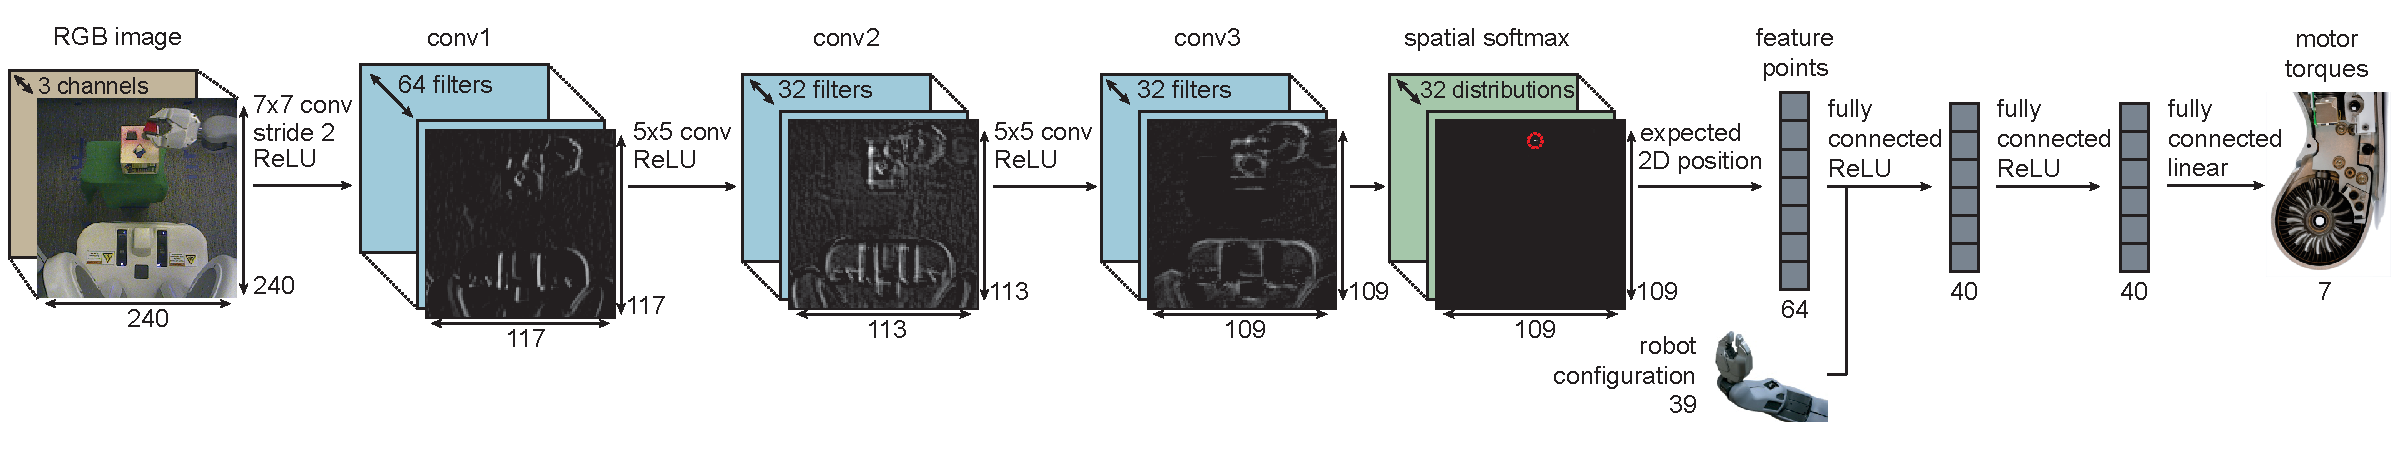
\includegraphics[width=\textwidth]{imgs/network_diagram.pdf}
%\end{subfigure}%
\vspace{-0.3in}
\caption{Visuomotor policy architecture. The network contains three convolutional layers, followed by a spatial softmax and an expected position layer that converts pixel-wise features to feature points, which are better suited for spatial computations. The points are concatenated with the robot configuration, then passed through three fully connected layers to produce the torques.
%Our network does not include pooling in order to preserve spatial information.
}
\vspace{-0.15in}
\label{fig:nn}
\end{figure*}

The aim of our method is to learn a policy $\policy_\params(\at|\ot)$ that specifies a distribution over actions $\at$ conditioned on the observation $\ot$, which includes a camera image and the configuration of the robot. The policy parameters $\params$ are optimized to minimize a cost function $\cost(\st,\at)$ over the course of a fixed-length episode. The actions $\at$ are the motor torques, and the state $\st$ includes the known robot configuration as well as (for example) the target position for an object placement task or the grasp pose. The latter information is not observed directly by the policy, and must be inferred from the camera image. We represent $\policy_\params(\at|\ot)$ as a Gaussian, with the mean given by a nonlinear function approximator. Since this function approximator needs to operate directly on raw images, we use convolutional neural networks (CNNs), which have enjoyed considerable success in computer vision \cite{ksh-incdc-12}. The architecture of our CNN is shown in Figure~\ref{fig:nn}. This network has 7 layers and around 92,000 parameters, which presents a tremendous challenge for standard policy search methods \cite{dnp-spsr-13}.

To handle this high dimensionality and the challenge of partial observability, we extend the framework of guided policy search. In guided policy search, the policy is trained with supervised learning, which scales well even to very high-dimensional function approximators. To construct the training set for supervised learning, we employ a trajectory-centric reinforcement learning method that finds good trajectories from a number of initial states. This phase does not require knowledge of the system dynamics, but does use the full state $\st$, which makes learning very efficient. For example, if the unobserved part of $\st$ is the position of a target object, such as the bottle, we can hold this object in the robot's left gripper, while the right arm performs the task. This type of instrumented training is a natural fit for many robotic tasks, where the training is performed in a controlled environment, but the final policy must be able to succeed ``in the wild.''

Na\"{i}ve supervised learning will often fail to produce a good policy, since a small mistake on the part of the policy will put it in states that are not part of the training, causing compounding errors. To avoid this problem, the training data must come from the policy's own state distribution \cite{rgb-rilsp-11}. We use BADMM \cite{wb-badmm-14} to adapt the trajectories to the policy, alternating between optimizing the policy to match the trajectories, and optimizing the trajectories to minimize cost and match the policy, such that at convergence, they have the same state distribution.


\subsection{Network Architecture}
\label{sec:policyarch}

Our visuomotor policy runs at 20 Hz on the robot, mapping monocular RGB images and the robot configurations to joint torques on a 7 DoF arm. The configuration includes the angles of the joints and the pose of the end-effector (defined by 3 points), as well as their velocities, but does not include the position of the target object or goal, which must be determined from the image. CNNs often use pooling to discard the locational information that is necessary to determine positions, since it is an irrelevant distractor for tasks such as object classification \cite{lgrn-cdbn-09}. Because locational information is important for control, our policy does not use pooling. Additionally, CNNs built for spatial tasks such as human pose estimation often also rely on the availability of location labels in image-space, such as hand-labeled keypoints~\cite{tjlb-jcngm-14}. We propose a novel CNN architecture capable of estimating spatial information from an image without direct supervision in image space. Our pose estimation experiments, discussed in Section~\ref{sec:training}, show that this network can learn useful visual features using only 3D positional information provided by the robot and no camera calibration. Furthermore, by training our network with guided policy search, it can acquire \emph{task-specific} visual features that improve policy performance.


Our network architecture is shown in Figure~\ref{fig:nn}. The visual processing layers of the network consist of three convolutional layers, each of which learns a bank of filters that are applied to patches centered on every pixel of its input. These filters form a hierarchy of local image features. Each convolutional layer is followed by a rectifying nonlinearity of the form $\responsepix=max(0,z_{cij})$ for each channel $\channel$ and each pixel coordinate $(i,j)$. The third convolutional layer contains $32$ response maps with resolution $109 \times 109$. These response maps are passed through a spatial softmax function of the form $\softmaxpix = {e^{\responsepix}}/{\sum_{i' j'}{e^{\responsepixprime}}}$.
%\[
%\softmaxpix = \frac{e^{\responsepix}}{\sum_{i' j'}{e^{\responsepixprime}}}.
%\]
Each output channel of the softmax is a probability distribution over the location of a feature in the image. To convert from this distribution to a spatial representation, the network calculates the expected image position of each feature, yielding a 2D coordinate for each channel. These feature points are concatenated with the robot's configuration and fed through two fully connected layers, each with 40 rectified units, followed by linear connections to the torques. The full visuomotor policy contains about 92,000 parameters, of which 86,000 are in the convolutional layers.

The spatial softmax and the expected position computation serve to convert pixel-wise representations in the convolutional layers to spatial coordinate representations, which can be manipulated by the fully connected layers into 3D positions or motor torques. The softmax also provides lateral inhibition, which suppresses low, erroneous activations.
%, only keeping strong activations that are more likely to be accurate.
This makes our policy more robust to distractors, providing generalization to novel visual variation. We compare our architecture with more standard alternatives in Section~\ref{sec:poseeval}.


\subsection{Training Data}
\label{sec:training}

\begin{wrapfigure}{r}{.3\columnwidth}
\vspace{-0.17in}
\hspace{-0.025\columnwidth}\includegraphics[width=0.32\columnwidth]{imgs/training_setup_sm.png}
\put(-41.00,65.00){\includegraphics[width=0.15\columnwidth,frame]{imgs/firstperson_training_setup.png}}
\vspace{-0.25in}
\end{wrapfigure}
We train the policy using the full state during the trajectory optimization phase, though the final policy acts under partial observations. This type of instrumented training is a natural choice for many robotics tasks, where the robot is trained under controlled conditions, but must then act intelligently in uncontrolled, real-world situations. In our tasks, the unobserved variables are the pose of a target object (e.g. the bottle on which a cap must be placed). During training, this target object is held in the robot's left gripper, while the robot's right arm performs the task, as shown above. This allows the robot to move the target through a range of known positions. The final visuomotor policy does not receive this position as input, but must instead use the camera images. The left arm is covered with cloth to prevent the policy from associating its appearance with the object's position.

While we can train the visuomotor policy entirely on the robot, the algorithm would spend a large number of iterations learning basic visual features and arm motions that can more efficiently be learned by themselves, before being incorporated into the policy. To speed up learning, we initialize both the vision layers in the policy and the trajectory distributions for guided policy search by leveraging the fully observed training setup. This initialization does not use any additional information that is not already available from the robot. To initialize the vision layers, the robot moves the target object through a range of random positions, recording the object's pose and camera images. This dataset is used to train a pose regression CNN, which consists of the same vision layers as the policy, followed by a fully connected layer that outputs the 3D points that define the target. Since the training set is still quite limited, we initialize the filters in the first layer with weights from the model of Szegedy et al. \cite{sljsr-gdwc-14}, which is trained on ImageNet~\cite{ddsll-lshid-09} classification. After training on pose regression, the weights in the convolutional layers are transferred to the policy CNN. This enables the robot to learn the appearance of the objects prior to learning the behavior.


%\begin{wrapfigure}{r}{.48\columnwidth}
\begin{wrapfigure}{r}{.4\columnwidth}
%\vspace{-0.15in}
%\includegraphics[height=0.65\columnwidth]{imgs/vgps_training_v2.png}
%\vspace{-0.32in}
\setlength{\unitlength}{0.5\columnwidth}
\begin{picture}(0.99,0.84) \linethickness{0.5pt}

\put(-0.04,-0.13){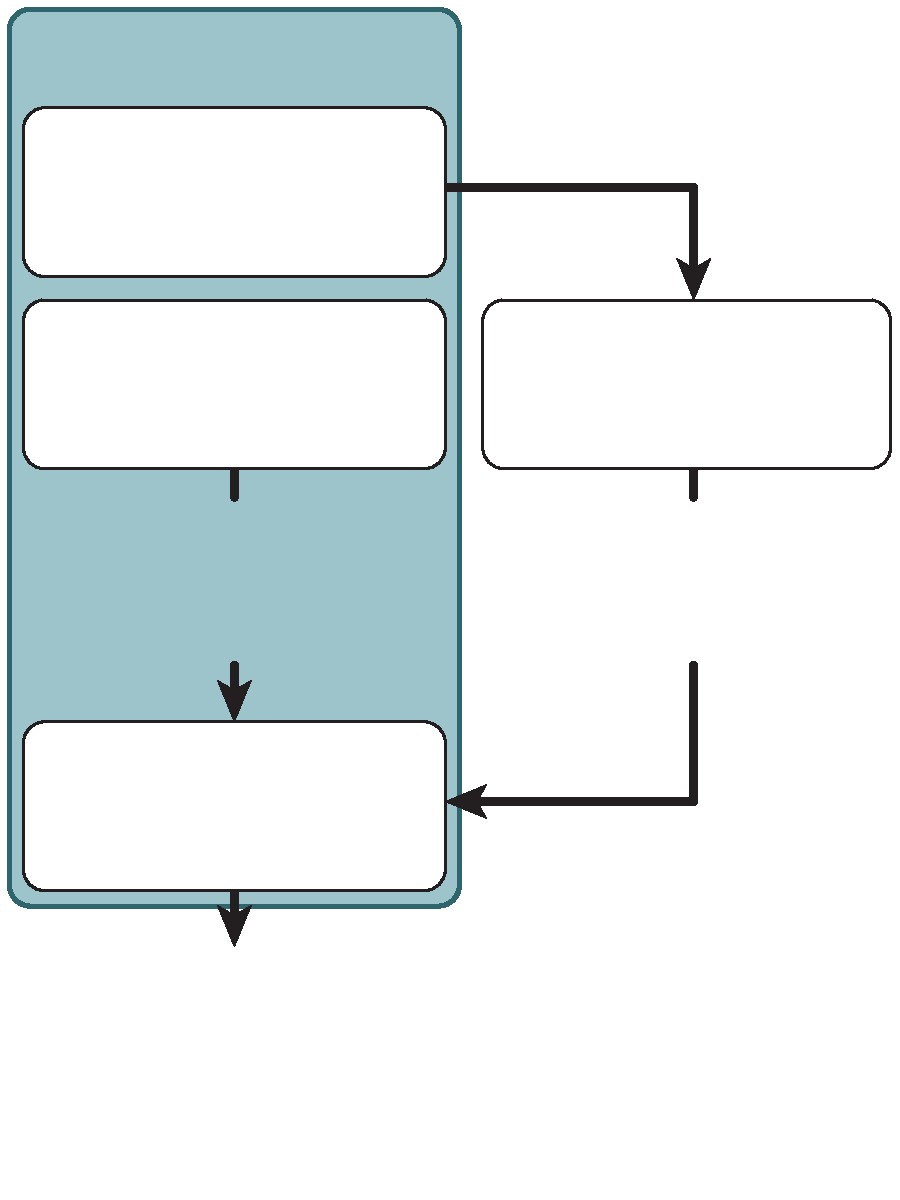
\includegraphics[width=0.4\columnwidth]{imgs/training_setup.pdf}}

\footnotesize{
\put(-0.015,0.87){requires robot}

\put(-0.005,0.78){collect visual}
\put(0.04,0.715){pose data}

\put(0.07,0.62){pretrain}
\put(0.025,0.55){trajectories}

\put(0.45,0.62){train pose}
\put(0.5,0.55){CNN}

\put(0.42,0.43){initial visual}
\put(0.48,0.36){features}

\put(0.105,0.43){initial}
\put(0.04,0.36){trajectories}

\put(0.03,0.24){end-to-end}
\put(0.06,0.17){training}

\put(0.085,0.04){policy}
}

\end{picture}
\vspace{-0.35in}

\end{wrapfigure}
To initialize the trajectories, we take 15 iterations of guided policy search without optimizing the visuomotor policy. This allows for much faster training in the early iterations, when the trajectories are not yet successful, and optimizing the full visuomotor policy is unnecessarily time consuming. Since we still want the trajectories to arrive at compatible strategies for each target position, we replace the visuomotor policy during these iterations with a small network that receives the full state. This network serves only to constrain the trajectories and avoid divergent behaviors from emerging for similar initial states, which would make subsequent policy learning difficult. As shown in the diagram above, the trajectories can be pre-trained in parallel with the vision layer pre-training, which does not require the robot.


After initialization, we train the full visuomotor policy with guided policy search. During the supervised policy optimization phase, the fully connected motor control layers are first optimized by themselves, since they are not initialized with pre-training. Then, the entire network is further optimized end-to-end. We found that this setup prevents the convolutional layers from forgetting the useful features learned during pre-training while still training all layers of the policy.

\section{Experimental Results}
\label{sec:results}

We evaluated our method by training policies for hanging a coat hanger on a clothes rack, inserting a block into a shape sorting cube, fitting the claw of a toy hammer under a nail with various grasps, and screwing on a bottle cap. The cost function for these tasks encourages low distance between three points on the end-effector and corresponding target points, low torques, and, for the bottle task, spinning the wrist. The equations for these cost functions follow prior work \cite{lwa-lnnpg-15}. The tasks are illustrated in Figure~\ref{fig:tasks}. Each task involved variation of about 10-20 cm in each direction in the position of the target object (the rack, shape sorting cube, nail, and bottle). In addition, the coat hanger and hammer tasks were trained with two and three grasps, respectively. All tasks used the same policy architecture and model parameters.

\begin{figure}
\setlength{\unitlength}{1.0\columnwidth}
\begin{picture}(1.0,0.55) \linethickness{0.5pt}

\put(0.0,0.04){\includegraphics[width=0.24\columnwidth]{imgs/hangerclose_sm.png}}
\put(0.0,0.29){\includegraphics[width=0.24\columnwidth]{imgs/hangerfar_sm.png}}

\put(0.25,0.04){\includegraphics[width=0.24\columnwidth]{trial_imgs/trap_bottomleft_start.png}}
\put(0.25,0.29){\includegraphics[width=0.24\columnwidth]{trial_imgs/trap_topright_start.png}}

\put(0.50,0.04){\includegraphics[width=0.24\columnwidth]{imgs/graspa_sm.png}}
\put(0.50,0.29){\includegraphics[width=0.24\columnwidth]{imgs/graspc_sm.png}}

\put(0.75,0.04){\includegraphics[width=0.24\columnwidth]{imgs/bottle_cropped_top_right.png}}
\put(0.75,0.29){\includegraphics[width=0.24\columnwidth]{imgs/bottle_cropped_bottom_left.png}}

\put(0.025,0.0){(a) hanger}
\put(0.3,0.0){(b) cube}
\put(0.525,0.0){(c) hammer}
\put(0.8,0.0){(d) bottle}

\end{picture}
\caption{Illustration of the tasks in our experiments, showing the variation in the position of the target for the hanger, cube, and bottle tasks, as well as two of the three grasps for the hammer, which also included variation in position (not shown).}
\label{fig:tasks}
\vspace{-0.2in}
\end{figure}

\subsection{Visuomotor Policy Generalization}

We evaluated the visuomotor policies in three conditions: (1) the training target positions and grasps, (2) new target positions not seen during training and, for the hammer, new grasps (spatial test), and (3) training positions with visual distractors (visual test). A selection of these experiments is shown in the supplementary video.\footnote{The video can be viewed at \url{http://sites.google.com/site/visuomotorpolicy}} For the visual test, the shape sorting cube was placed on a table rather than held in the gripper, the coat hanger was placed on a rack with clothes, and the bottle and hammer tasks were done in the presence of clutter. Illustrations of this test are shown in Figure~\ref{fig:traintest}.


The success rates for each test are shown in Table~\ref{tbl:results}. We compared to two baselines, both of which train the vision layers in advance for pose prediction, instead of training the entire policy end-to-end. The features baseline discards the last layer of the pose predictor and uses the feature points, resulting in the same architecture as our policy, while the prediction baseline feeds the predicted pose into the control layers.

The pose prediction baseline is analogous to a standard modular approach to policy learning, where the vision system is first trained to localize the target, and the policy is trained on top of it. This variant achieves poor performance, because although the pose is accurate to about 1 cm, this is insufficient for such precise tasks. As shown in the video, the shape sorting cube and bottle cap insertions have tolerances of just a few millimeters. Such accuracy is difficult to achieve even with calibrated cameras and checkerboards. Indeed, prior work has reported that the PR2 can maintain a camera to end effector accuracy of about 2 cm during open loop motion \cite{mwgcm-adopi-10}. This suggests that the failure of this baseline is not atypical, and that our visuomotor policies are learning visual features and control strategies that improve the robot's accuracy.

% As reported in prior work, the PR2 is only able to maintain a camera to end effector accuracy of about 2 cm during an open loop manipulation task with standard vision techniques based on checkerboards \cite{mwgcm-adopi-10}.

When provided with pose estimation features, the policy has more freedom in how it uses the visual information, and achieves somewhat higher success rates. However, full end-to-end training performs significantly better, achieving high accuracy even on the challenging bottle task, and successfully adapting to the variety of grasps on the hammer task. This suggests that, although the vision layer pre-training is clearly beneficial for reducing computation time, it is not sufficient by itself for discovering good features for visuomotor policies.


\begin{figure}
\setlength{\unitlength}{0.5\columnwidth}
\begin{picture}(1.99,1.06) \linethickness{0.5pt}

\put(0.08,0.56){\includegraphics[width=0.23\columnwidth]{trial_imgs/hanger_firstperson_close_train.png}}
\put(0.08,0.08){\includegraphics[width=0.23\columnwidth]{trial_imgs/hanger_firstperson_close.png}}

\put(0.56,0.56){\includegraphics[width=0.23\columnwidth]{trial_imgs/trap_topright_end.png}}
\put(0.56,0.08){\includegraphics[width=0.23\columnwidth]{trial_imgs/trapezoid_firstperson.png}}

\put(1.04,0.56){\includegraphics[width=0.23\columnwidth]{trial_imgs/hammer_firstperson_grasp1_train_crop.png}}
\put(1.04,0.08){\includegraphics[width=0.23\columnwidth]{trial_imgs/hammer_firstperson_grasp1_crop.png}}

\put(1.52,0.56){\includegraphics[width=0.23\columnwidth]{trial_imgs/bottle_firstperson_train_crop.png}}
\put(1.52,0.08){\includegraphics[width=0.23\columnwidth]{trial_imgs/bottle_firstperson_test_crop.png}}

\put(0.12,0.0){(a) hanger}
\put(0.65,0.0){(b) cube}
\put(1.08,0.0){(c) hammer}
\put(1.61,0.0){(d) bottle}
\put(0.0,0.69){\rotatebox{90}{training}}
\put(0.0,0.15){\rotatebox{90}{visual test}}

\end{picture}
\caption{Training and visual test scenes as seen by the policy at the ends of successful episodes. The hammer and bottle images were cropped for visualization only.
}
\label{fig:traintest}
\vspace{-0.0in}
\end{figure}


\begin{table}[h!]
{\footnotesize
  \begin{center}
    \begin{tabular}{| l | l | l | l |}
    \hline
    coat hanger & training (18) & spatial test (24) & visual test (18)\\
    \hline
    end-to-end training & {\bf 100\%} & {\bf 100\%} & {\bf 100\%} \\
    \hline
    pose features & 88.9\% & 87.5\% & 83.3\% \\
    \hline
    pose prediction & 55.6\% & 58.3\% & 66.7\%  \\
    \hline
    \hline
    shape sorting cube & training (27) & spatial test (36) & visual test (40) \\
    \hline
    end-to-end training & {\bf 96.3\%} & {\bf 91.7\%} & {\bf 87.5\%} \\
    \hline
    pose features & 70.4\% & 83.3\% & 40\%\\
    \hline
    pose prediction & 0\% & 0\% & n/a\\
    \hline
    \hline
    toy claw hammer & training (45) & spatial test (60) & visual test (60) \\
    \hline
    end-to-end training & {\bf 91.1\%} & {\bf 86.7\%} & {\bf 78.3\%} \\
    \hline
    pose features & 62.2\% & 75.0\% & 53.3\%\\
    \hline
    pose prediction & 8.9\% & 18.3\% & n/a\\
    \hline
    \hline
    bottle cap & training (27) & spatial test (12) & visual test (40) \\
    \hline
    end-to-end training & {\bf 88.9\%} & {\bf 83.3\%} & {\bf 62.5\%}\\
    \hline
    pose features & 55.6\% & 58.3\% & 27.5\%\\
    \hline
    \end{tabular}
  \end{center}
}
\vspace{-0.1in}
  \caption{Success rates on training positions, on novel test positions, and in the presence of visual distractors. The number of trials per test is shown in parentheses.}
  \label{tbl:results}
\vspace{-0.15in}
\end{table}

The policies exhibit moderate tolerance to distractors that are visually separated from the target object. However, as expected, they tend to perform poorly under drastic changes to the backdrop, or when the distractors are adjacent to or occluding the manipulated objects, as shown in the supplementary video. In future work, this could be mitigated by varying the scene at training time, or by artificially augmenting the image samples with synthetic transformations, as discussed in prior work in computer vision \cite{ssp-bpcnn-03}.

\subsection{Features Learned with End-to-End Training}

\begin{figure}
\setlength{\unitlength}{0.5\columnwidth}
\begin{picture}(1.99,1.15) \linethickness{0.5pt}

\put(0.0,0.555){\includegraphics[width=0.245\columnwidth]{imgs/trial_conv3_4041_23.png}}
\put(0.0,0.08){\includegraphics[width=0.245\columnwidth]{imgs/trial_conv3_4041_24.png}}
\put(0.47,0.555){\includegraphics[width=0.245\columnwidth]{imgs/trial_softmax_4041_23_cyan.png}}
\put(0.47,0.08){\includegraphics[width=0.245\columnwidth]{imgs/trial_softmax_4041_24_cyan.png}}
\put(.98,0.07){\includegraphics[width=0.5\columnwidth]{imgs/points_41_comparison_cyan.png}}
\put(0.08,0.0){(a) conv3}
\put(0.53,0.0){(b) softmax}
\put(1.22,0.0){(c) feature points}

\end{picture}
\caption{Feature points learned by the shape sorting cube policy. Two of the 32 conv3 response maps are shown in (a), and the corresponding softmax distributions are displayed in (b). In (c), we show the output feature points for this input image in blue, while the feature points of the pose prediction network are shown in red. The end-to-end trained model discovers more feature points on the cube and the gripper.}
\label{fig:comppoints}
\vspace{-0.2in}
\end{figure}

In Figure~\ref{fig:comppoints}, we compare the feature points learned through guided policy search to those learned by a CNN trained for pose prediction. After end-to-end training, the policy acquired a distinctly different set of feature points compared to the pose prediction CNN used for initialization. The end-to-end trained model finds more feature points on task-relevant objects and fewer points on background objects. This suggests that the policy improves its performance by acquiring \emph{task-specific} visual features that differ from those learned for object localization. We further analyze the features learned by our policies in the supplementary appendix.

\subsection{CNN Architecture Evaluation}
\label{sec:poseeval}

To evaluate the visual processing portion of our architecture, we measured its accuracy on the pose estimation pre-training task discussed in Section~\ref{sec:training}. We compare to a network where the fixed transformation from the softmax to the feature points is replaced with a conventional learned fully connected layer, as well as to networks that omit the softmax and use $3\times 3$ max pooling with stride $2$ at the first two layers. These alternative architectures have many more parameters, since the new fully connected layer takes as input the entire bank of response maps from the third convolutional layer.
The results in Table~\ref{tbl:posebaseline} indicate that using the softmax and the fixed transformation from the softmax output to the spatial feature representation improves pose estimation accuracy and reduces overfitting. Our network is able to outperform the more standard architectures because it is forced by the softmax and expected position layers to learn feature points, which provide a concise representation suitable for spatial inference. The lower number of parameters also results in an easier optimization and reduces overfitting.


\begin{table}[h!]
  \begin{center}
    \begin{tabular}{| l | l | l | }
    \hline
    network architecture & training error (cm) & test error (cm)  \\
    \hline
    softmax + feature points ({\bf ours}) & {\bf 1.14 $\pm$ 1.67}  & {\bf 1.30 $\pm$ 0.73} \\
    \hline
    softmax + fully connected layer & 2.27 $\pm$ 1.70 & 2.59 $\pm$ 1.19 \\
    \hline
    fully connected layer & 4.65 $\pm$ 2.90  & 4.75 $\pm$ 2.29  \\
    \hline
    max-pooling + fully connected & 2.89 $\pm$ 2.08 & 3.71 $\pm$ 1.73 \\
    \hline
    \end{tabular}
  \end{center}
\vspace{-0.1in}
  \caption{Average pose estimation accuracy and standard deviation with various architectures, measured as average Euclidean error for the three target points in 3D, with ground truth determined by forward kinematics from the left arm.
}
  \label{tbl:posebaseline}
\vspace{-0.05in}
\end{table}

\subsection{Implementation and Computational Performance}

CNN training was implemented using the Caffe~\cite{jsdkl-caffe-14} deep learning library. Each visuomotor policy required 3-4 hours of training time: 20-30 minutes for the pose prediction data collection on the robot, 40-60 minutes for the fully observed trajectory pre-training on the robot and offline pose pre-training (which can be done in parallel), and between 1.5 and 2.5 hours for end-to-end training with guided policy search. The coat hanger task required two iterations of guided policy search, the shape sorting cube and the hammer required three, and the bottle task required four. Training time was dominated by computation rather than robot interaction time, and we expect significant speedup from a more efficient implementation.

\section{Discussion and Future Work}
\label{sec:conclusion}

In this paper, we presented a method for learning robotic control policies that use raw input from a monocular camera. These policies are represented by a novel convolutional neural network architecture, and can be trained end-to-end using our partially observed guided policy search algorithm, which decomposes the policy search problem in a trajectory optimization phase that uses full state information and a supervised learning phase that only uses partial observations. This decomposition allows us to leverage state-of-the-art tools from supervised learning, making it straightforward to optimize extremely high-dimensional policies. Our experimental results show that our method can execute complex manipulation skills, and that end-to-end training produces significant improvements in policy performance compared to using fixed vision layers trained for pose prediction.

Although we demonstrate moderate generalization over variations in the scene, our current method does not generalize to dramatically different settings, especially when visual distractors occlude the manipulated object or break up its silhouette in ways that differ from the training. The success of CNNs on exceedingly challenging vision tasks suggests that this class of models is capable of learning invariance to irrelevant distractor features \cite{gddm-fhaod-13,ksh-incdc-12,tjlb-jcngm-14}, and in principle this issue can be addressed by training the policy in a variety of environments, though this poses certain logistical challenges. More practical alternatives that could be explored in future work include simultaneously training the policy on multiple robots, each of which is located in a different environment, developing more sophisticated regularization and pre-training techniques to avoid overfitting, and introducing artificial data augmentation to encourage the policy to be invariant to irrelevant clutter. However, even without these improvements, our method has numerous applications in, for example, an industrial setting where the robot must repeatedly and efficiently perform a task that requires visual feedback under moderate variation in background and clutter conditions.

In future work, we hope to explore more complex policy architectures, such as recurrent policies that can deal with extensive occlusions by keeping a memory of past observations. We also hope to extend our method to a wider range of tasks that can benefit from visual input, as well as a variety of other rich sensory modalities, including haptic input from pressure sensors and auditory input. With a wider range of sensory modalities, end-to-end training of sensorimotor policies will become increasingly important: while it is often straightforward to imagine how vision might help to localize the position of an object in the scene, it is much less apparent how sound can be integrated into robotic control. A learned sensorimotor policy would be able to naturally integrate a wide range of modalities and utilize them to directly aid in control.

%\section*{Acknowledgments}

\bibliographystyle{plainnat}
\bibliography{references}

\clearpage
\subsection{Feature Point Analysis}

The visual processing layers of our architecture automatically learn features points using the fixed transformation from the softmax to spatial coordinates. These feature points encapsulate all of the visual information received by the motor layers of the policy. In Figure~\ref{fig:ptssupp}, we show the features points discovered by our visuomotor policy through guided policy search. Each policy learns features on the target object and the robot manipulator, both clearly relevant to task execution. The policy tends to pick out robust, distinctive features on the objects, such as the left pole of the clothes rack, the left corners of the shape-sorting cube, the bottom-left corner of the toy tool bench, and the edges of the bottle.

In Figure~\ref{fig:points_comparison_supp}, we compare the feature points learned through guided policy search to those learned by a CNN trained for pose prediction. Note that in all tasks, the end-to-end trained model produces fewer points on the background compared to the model trained on object pose. In the bottle task, the end-to-end trained policy outputs points on both sides of the bottle, including one on the cap, while the pose prediction network only finds points on the right edge of the bottle.
%For example, the end-to-end trained model outputs only one feature point on the hanger task backdrop compared to four outputted by the pose prediction network.

The feature point representation is very simple, since it assumes that the learned features are present at all times. While this is a drastic simplification, both the pose predictor and the policy still achieve good results. A more flexible architecture that still learns a concise feature point representation could further improve policy performance. We hope to explore this in future work.

\begin{figure*}
\setlength{\unitlength}{1.0\columnwidth}
\begin{picture}(2.0,1.5) \linethickness{0.5pt}

\put(0.0,0.91){\includegraphics[width=0.49\columnwidth]{imgs/hanger_pts0.png}}
\put(0.0,0.46){\includegraphics[width=0.49\columnwidth]{imgs/hanger_pts1.png}}
\put(0.0,0.01){\includegraphics[width=0.49\columnwidth]{imgs/hanger_pts2.png}}

\put(0.5,0.91){\includegraphics[width=0.49\columnwidth]{imgs/cube_pts0.png}}
\put(0.5,0.46){\includegraphics[width=0.49\columnwidth]{imgs/cube_pts1.png}}
\put(0.5,0.01){\includegraphics[width=0.49\columnwidth]{imgs/cube_pts2.png}}

\put(1.0,0.91){\includegraphics[width=0.49\columnwidth]{imgs/hammer_pts2.png}}
\put(1.0,0.46){\includegraphics[width=0.49\columnwidth]{imgs/hammer_pts1.png}}
\put(1.0,0.01){\includegraphics[width=0.49\columnwidth]{imgs/hammer_pts0.png}}

\put(1.5,0.91){\includegraphics[width=0.49\columnwidth]{imgs/bottle_pts0.png}}
\put(1.5,0.46){\includegraphics[width=0.49\columnwidth]{imgs/bottle_pts1.png}}
\put(1.5,0.01){\includegraphics[width=0.49\columnwidth]{imgs/bottle_pts2.png}}

\put(0.15,-0.01){(a) hanger}
\put(0.67,-0.01){(b) cube}
\put(1.15,-0.01){(c) hammer}
\put(1.68,-0.01){(d) bottle}

\end{picture}
\caption{Feature points tracked by the policy during task execution for each of the four tasks. Each feature point is displayed in a different random color, with consistent coloring across images. The policy finds features on the target object and the robot gripper and arm. In the bottle cap task, note that the policy correctly ignores the distractor bottle in the background, even though it was not present during training.}
\label{fig:ptssupp}
%\vspace{-1.2in}
%\vspace{-0.2in}
\end{figure*}

\begin{figure*}
\setlength{\unitlength}{1.0\columnwidth}
\begin{picture}(2.0,0.5) \linethickness{0.5pt}

\put(0.0,0.01){\includegraphics[width=0.49\columnwidth]{imgs/comparepoints_hanger.png}}

\put(0.5,0.01){\includegraphics[width=0.49\columnwidth]{imgs/points_41_comparison.png}}

\put(1.0,0.01){\includegraphics[width=0.49\columnwidth]{imgs/comparepoints_hammer.png}}

\put(1.5,0.01){\includegraphics[width=0.49\columnwidth]{imgs/comparepoints_bottle.png}}

\put(0.15,-0.01){(a) hanger}
\put(0.67,-0.01){(b) cube}
\put(1.15,-0.01){(c) hammer}
\put(1.68,-0.01){(d) bottle}

\end{picture}
        \caption{Feature points learned for each task. For each input image, the feature points produced by the policy are shown in blue, while the feature points of the pose prediction network are shown in red. The end-to-end trained policy tends to discover more feature points on the target object and the robot arm than the pose prediction network.}
	\label{fig:points_comparison_supp}
\end{figure*}



\end{document}


